 \subsection*{1.}
 \FloatBarrier
 We record the default options for the computations in this exercise in \cref{Defaults} and see that indeed the size of the matrix is the only quantity that changes.
 \begin{table}[h!]
\centering
\begin{tabular}{|l|l|l|}
\hline
\textbf{Dimension} & \textbf{Default KSP/PC} & \textbf{Matrix Size} \\ \hline
1D & GMRES / ILU (0 fill) & $9$ \\ \hline
2D & GMRES / ILU (0 fill) & $9 \times 9$ \\ \hline
3D & GMRES / ILU (0 fill) & $9 \times 9 \times 9$ \\ \hline
\end{tabular}
\caption{Default KSP, PC options and Matrix Size for 1D, 2D, and 3D problems.}
\label{Defaults}
\end{table}


\FloatBarrier

\subsection*{2.}
\FloatBarrier
We record the required data in \cref{performance}.
\begin{table}[h!]
\centering
\begin{tabular}{|l|l|l|l|l|}
\hline
\textbf{Dimension} & \textbf{Wall-clock Time (s)} & \textbf{FLOPS/sec} & \textbf{Error $\|u-u_{exact}\|_\infty$} & \textbf{KSP Iterations} \\ \hline
1D & 0.0224 & $2.59 \times 10^4$ & 0.00110617 & 1 \\ \hline
2D & 0.0275 & $4.94 \times 10^6$ & 0.000221974 & 11 \\ \hline
3D & 0.0707 & $5.56 \times 10^7$ & 0.0215725 & 15 \\ \hline
\end{tabular}
\caption{Performance metrics for 1D, 2D, and 3D cases.}
\label{performance}
\end{table}


\FloatBarrier

\subsection*{3.}
\FloatBarrier
In this exercise we plot the assembled matrices in 1D, 2D, and 3D. In the 1D matrix one sees the typical structure of the 1D laplacian, $2$ on the diagonals, $-1$ on the off diagonals. Since the stencils become larger in higher dimension, one row contains more values in 2D and 3D than in 1D. However, we also see that the matrices are still sparse. for the same $\Delta x$, the 2D and 3D matrices are much larger since they contain much more grid points. The pattern we see in the plot depends on the ordering of the gridpoints in the linear system and this is not the only possible choice.

\begin{figure}[h!]
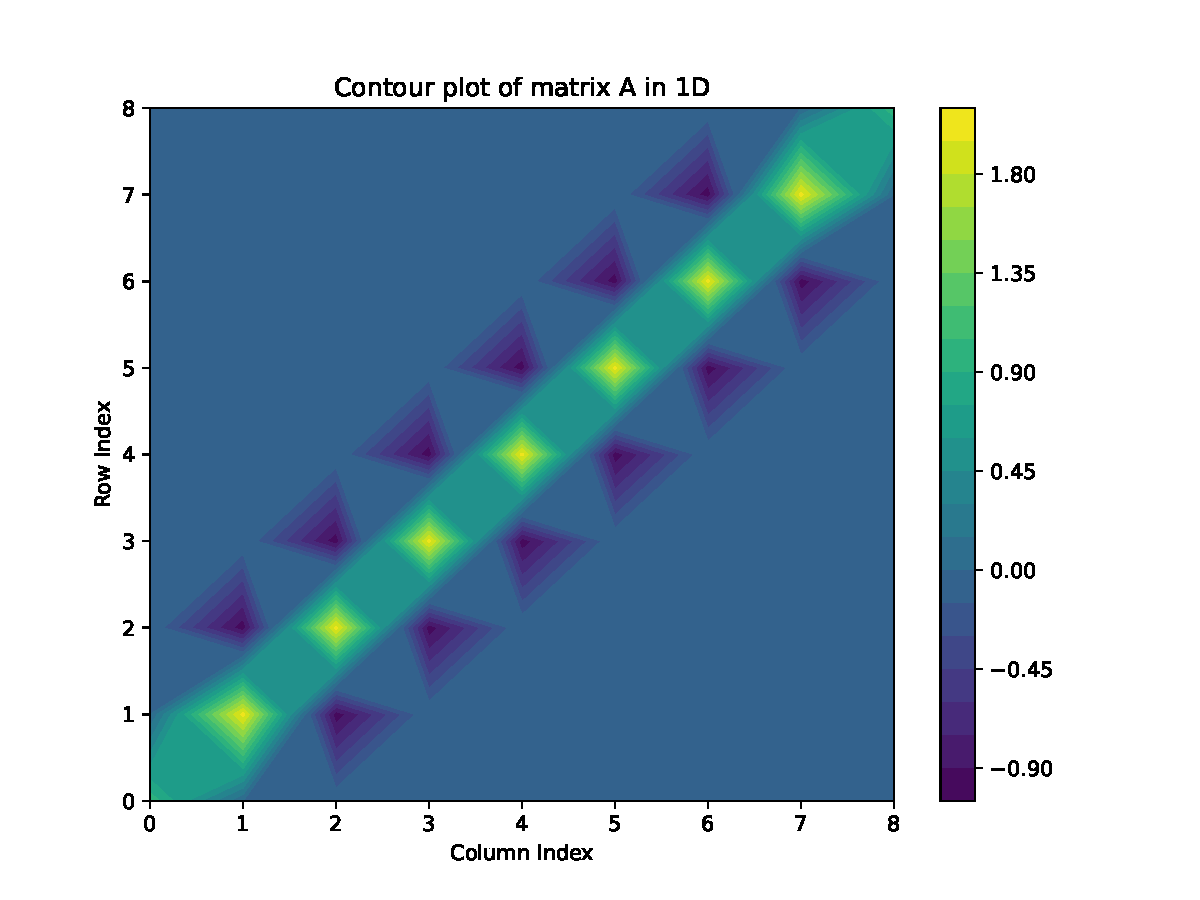
\includegraphics[width=\textwidth]{contour_plot1D.pdf}
\caption{1D Contour plot of matrix}
\label{fig:contour1D}
\end{figure}

\begin{figure}[h!]
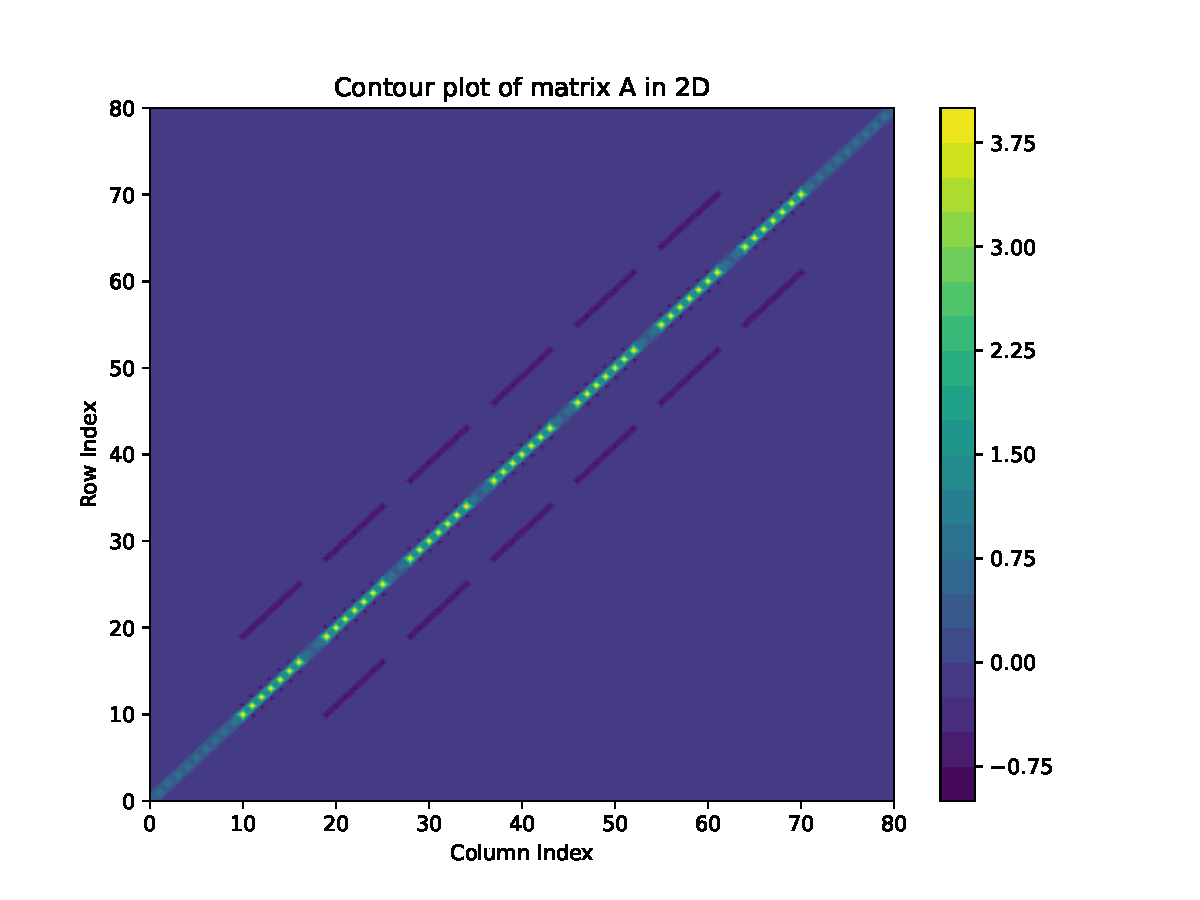
\includegraphics[width=\textwidth]{contour_plot2D.pdf}
\caption{2D Contour plot of matrix}
\label{fig:contour1D}
\end{figure}

\begin{figure}[h!]
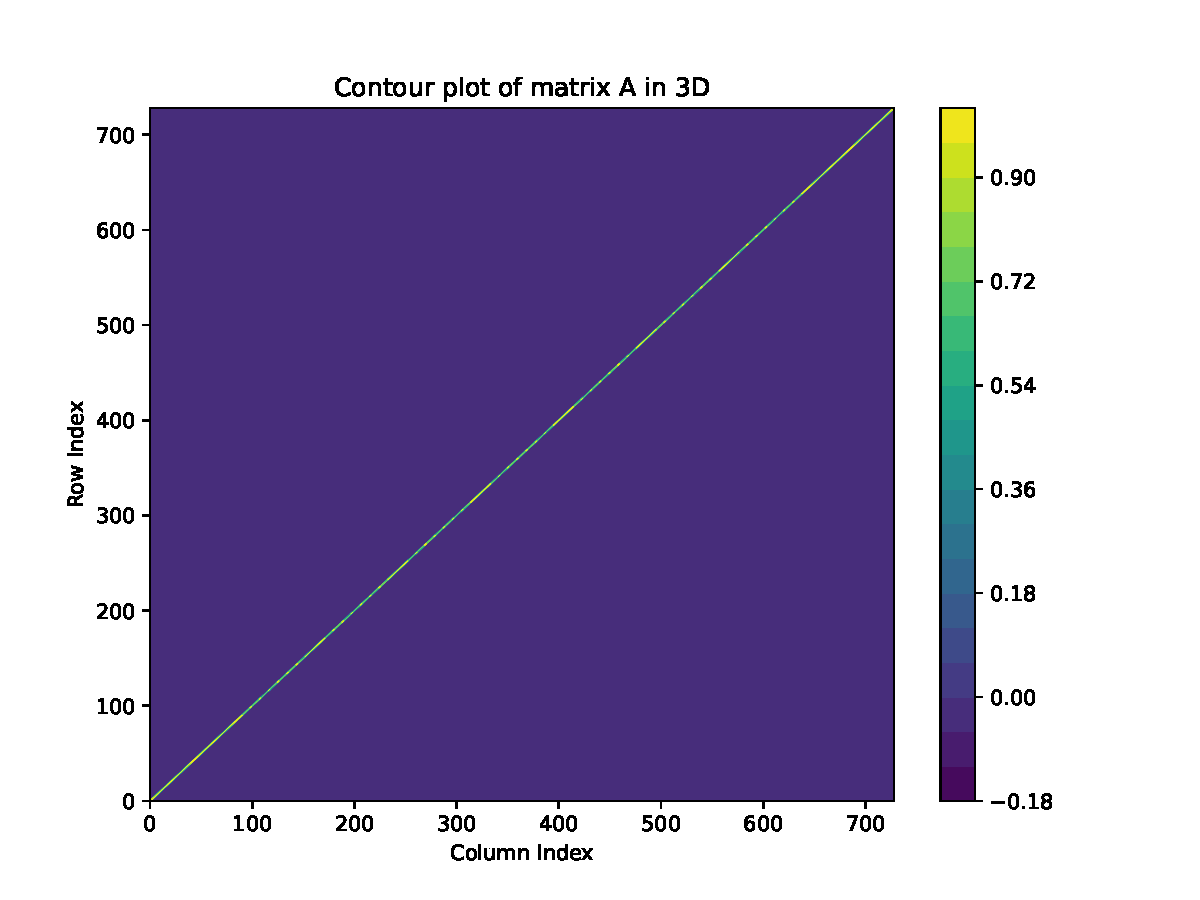
\includegraphics[width=\textwidth]{contour_plot3D.pdf}
\caption{3D Contour plot of matrix}
\label{fig:contour1D}
\end{figure}


\FloatBarrier


\subsection*{4.}
\FloatBarrier
The KSP solver terminates after one iteration. The residual norm can be seen in \cref{iters}. Since the numerical error in the infinity norm is given by 0.00110617, we see that the residual error is much smaller. Hence, the error made through discretising (and not the one made when approximating the solution to the linear system) dominates the overall numerical error here.
\begin{table}[h!]
\centering
\begin{tabular}{|l|l|}
\hline
\textbf{Iteration} & \textbf{Residual Norm} \\ \hline
0 & $6.143 \times 10^{-1}$ \\ \hline
1 & $7.765 \times 10^{-17}$ \\ \hline
\end{tabular}
\caption{KSP Iterations and Residual Norms. Error $\|u-u_{exact}\|_\infty = 0.00110617$.}
\label{iters}
\end{table}



\FloatBarrier

\subsection*{5.}
\FloatBarrier
We record the required Eigenvalues in \Cref{evals}.
\begin{table}[h!]
\centering
\begin{tabular}{|l|l|}
\hline
\textbf{Iteration} & \textbf{Eigenvalue} \\ \hline
0 & 0.328089 \\ \hline
1 & 0.51186 \\ \hline
2 & 0.548359 \\ \hline
3 & 0.661475 \\ \hline
4 & 0.785197 \\ \hline
5 & 0.898367 \\ \hline
6 & 1.00172 \\ \hline
7 & 1.06566 \\ \hline
\end{tabular}
\caption{Eigenvalues computed in successive iterations.}
\label{evals}
\end{table}




\FloatBarrier


\subsection*{6.}
\FloatBarrier
We collect in \Cref{errors} the grid sizes, number of KSP iterations, the infinity norm error, the 1-norm error, the 2-norm error and their normalized variants. If $n$ is the dimension of the vector, then we need to normalize the 1-norm by dividing by $n$ and the 2-norm by dividing by $\sqrt{n}$ to obtain a reasonable error metric. This is because
\[
\norm{\cdot}_{1} \leq n \norm{\cdot}_{\infty}
\]
and
\[
\norm{\cdot}_2 \leq \sqrt{n} \norm{\cdot}_{\infty}
\]
and because after normalizations these metrics become discretizations of the $L^1$ and $L^2$ norms for functions. In \Cref{rates} we divide the error of one discretization by the error of the next coarser discretization. We see that overall that the respective value is about $4$ which is what we need to confirm the convergence rate, since the truncation error of the PDE is expected to be reduced by a factor of 4 every time we double the resolution. We also observe that we need much more KSP iterations with increasing size of the matrix.

\begin{table}[h!]
\hspace{-2cm}\begin{tabular}{|c|c|c|c|c|c|c|}
\hline
\textbf{Grid Size} & \textbf{Iterations} & \textbf{$\|u-u_{\text{exact}}\|_{\infty}$} & \textbf{$\|u-u_{\text{exact}}\|_1$} & \textbf{$\|u-u_{\text{exact}}\|_2$} & \textbf{Normalized 1-norm} & \textbf{Normalized 2-norm} \\ \hline
9x9     & 8   & 0.000763959 & 0.0211785 & 0.00329941 & 2.6212e-04 & 3.6653e-04 \\ \hline
17x17   & 12  & 0.000196764 & 0.0216913 & 0.00164961 & 7.4938e-05 & 1.2146e-04 \\ \hline
33x33   & 23  & 4.91557e-05 & 0.0218203 & 0.000824732 & 2.2506e-05 & 4.5323e-05 \\ \hline
65x65   & 56  & 1.29719e-05 & 0.0227638 & 0.000430681 & 8.4922e-06 & 1.5704e-05 \\ \hline
129x129 & 174 & 3.76924e-06 & 0.0256992 & 0.000245575 & 1.5412e-06 & 3.1172e-06 \\ \hline
\end{tabular}
\caption{Grid Size vs. Error and Iterations}
\label{errors}
\end{table}

\begin{table}[h!]
\centering
\begin{tabular}{|c|c|c|c|c|c|}
\hline
\textbf{Grid Size} & \textbf{Infinity Norm} & \textbf{1-Norm} & \textbf{2-Norm} & \textbf{Normalized 1-Norm} & \textbf{Normalized 2-Norm} \\ \hline
9x9     &        &        &        &        &        \\ \hline
17x17   & 3.882 & 0.9764 & 1.999 & 3.496 & 3.016 \\ \hline
33x33   & 4.003 & 0.995 & 2.000 & 3.329 & 2.678 \\ \hline
65x65   & 3.788 & 0.958 & 1.915 & 2.648 & 2.882 \\ \hline
129x129 & 3.442 & 0.885 & 1.753 & 5.510 & 5.037 \\ \hline
\end{tabular}
\caption{Convergence Rates}
\label{rates}
\end{table}






\FloatBarrier

\subsection*{7.}
\FloatBarrier
We print the condition number with respect to the 2-norm for the matrices in the previous discussion in \Cref{condnom}. This can be done by dividing the largest by the smallest Eigenvalue $\frac{\lambda_{max}}{\lambda_{min}}$. We computed approximations of these Eigenvalues in a previous exercise, when we listed them in the KSP iteration. We see that with growing size the matrices have larger condition numbers. This fits very well to our results on the convergence from the previous exercise, as we need much more KSP iterations for larger matrices, and the condition number describes how strong numerical errors propagate, i.e. how good a linear system can be solved.
\begin{table}[h!]
\centering
\begin{tabular}{|c|c|}
\hline
\textbf{Grid Size} & \textbf{Condition Number} \\ \hline
9x9     & 3.249 \\ \hline
17x17   & 8.377 \\ \hline
33x33   & 24.126 \\ \hline
65x65   & 50.329 \\ \hline
129x129 & 89.345 \\ \hline
\end{tabular}
\caption{Condition Numbers}
\label{condnom}
\end{table}




\FloatBarrier

\subsection*{8.}
\FloatBarrier
We record the results of our computations of numerical errors for different combinations of gridsizes and relative tolerances in \Cref{rtols}. We observe that for certain grid sizes it does not make sense to put effort in reaching very high accuracy in the KSP iteration because at some point the truncation error dominates and we obtain no further improvements by doing so.
\begin{table}[h!]
\centering
\begin{tabular}{|c|c|c|c|}
\hline
\textbf{Grid Size} & \textbf{RTOL = 1e-1} & \textbf{RTOL = 1e-5} & \textbf{RTOL = 1e-10} \\ \hline
$9 \times 9 \times 9$   & 0.00139236  & 0.000169304 & 0.000169304 \\ \hline
$17 \times 17 \times 17$ &0.00168387 & 4.2181e-05 & 4.21805e-05 \\ \hline
$33 \times 33 \times 33$ & 0.00146642 & 1.05899e-05 & 1.05776e-05 \\ \hline
\end{tabular}
\caption{Numerical error in infinity norm for different grid sizes and relative tolerances.}
\label{rtols}
\end{table}

\subsection*{9.}
\underline{1D grid:} The Laplacian in 1D is given by the second derivative
\[
\Delta \varphi = \frac{\partial^2 \varphi}{\partial x^2}.
\]
Using forward and backward finite difference approximations for one derivative, we obtain
\[
\varphi'(x) \approx \frac{\varphi(x + h) - \varphi(x)}{h}
\]
\[
\varphi'(x) \approx \frac{\varphi(x) - \varphi(x - h)}{h}
\]
Then we use the again finite differences to approximate the second derivative
\[
\varphi''(x) \approx \frac{\varphi'(x + h/2) - \varphi'(x - h/2)}{h} \approx \frac{\frac{\varphi(x + h) - \varphi(x)}{h} - \frac{\varphi(x) - \varphi(x - h)}{h}}{h} \approx \frac{\varphi(x + h) - 2\varphi(x) + \varphi(x - h)}{h^2}.
\]
Scaling now by $h^2$ gives $h^2 \varphi''(x) \approx \varphi(x + h) - 2\varphi(x) + \varphi(x - h)$. Renaming $\varphi_i := \varphi_i(x), \; \varphi_{i - 1} := \varphi(x - h), \; \varphi_{i + 1} := \varphi(x + h)$ gives the discrete Laplacian
\[
h^2 \Delta \varphi_i = \varphi_{i - 1} - 2\varphi_i + \varphi_{i + 1}.
\]
\\

\underline{3D grid:}
The Laplacian in 3D is given by
\[
\Delta \varphi = \frac{\partial^2 \varphi}{\partial x^2} + \frac{\partial^2 \varphi}{\partial y^2} + \frac{\partial^2 \varphi}{\partial z^2}.
\]

For the \(x\)-derivative we obtain the finite difference:
\[
\varphi_x'(x) \approx \frac{\varphi(x + h_x, y, z) - \varphi(x, y, z)}{h_x},
\]
\[
\varphi_x'(x) \approx \frac{\varphi(x, y, z) - \varphi(x - h_x, y, z)}{h_x}
\]
and hence iteratively
\[
\varphi_{xx}''(x) \approx \frac{\frac{\varphi(x + h_x, y, z) - \varphi(x, y, z)}{h_x} - \frac{\varphi(x, y, z) - \varphi(x - h_x, y, z)}{h_x}}{h_x}
= \frac{\varphi(x + h_x, y, z) - 2\varphi(x, y, z) + \varphi(x - h_x, y, z)}{h_x^2}.
\]

Similarly, we obtain for \(y\)- and \(z\)-derivatives:

\[
\varphi_{yy}''(y) \approx \frac{\varphi(x, y + h_y, z) - 2\varphi(x, y, z) + \varphi(x, y - h_y, z)}{h_y^2}
\]

\[
\varphi_{zz}''(z) \approx \frac{\varphi(x, y, z + h_z) - 2\varphi(x, y, z) + \varphi(x, y, z - h_z)}{h_z^2}.
\]

Substituting this into the first equation gives

\begin{align*}
\Delta \varphi \approx & \; \frac{\varphi(x + h_x, y, z) - 2\varphi(x, y, z) + \varphi(x - h_x, y, z)}{h_x^2} \\
& \; + \frac{\varphi(x, y + h_y, z) - 2\varphi(x, y, z) + \varphi(x, y - h_y, z)}{h_y^2} \\
& \; + \frac{\varphi(x, y, z + h_z) - 2\varphi(x, y, z) + \varphi(x, y, z - h_z)}{h_z^2}.
\end{align*}

Renaming the function values into $\varphi_{ijk}$ as in the 1D case and scaling by \(h_x h_y h_z\) gives:

\begin{align*}
h_x h_y h_z \Delta \varphi_{ijk} \approx
&\;  h_y h_z (\varphi_{i+1, j, k} - 2\varphi_{i, j, k} + \varphi_{i-1, j, k}) \\
& \; + h_x h_z (\varphi_{i, j+1, k} - 2\varphi_{i, j, k} + \varphi_{i, j-1, k}) \\
&\; + h_x h_y (\varphi_{i, j, k+1} - 2\varphi_{i, j, k} + \varphi_{i, j, k-1}).
\end{align*}


\FloatBarrier





